\documentclass{article}

\title{AES 규격}
\author{김동현(wlswudpdlf31@kookmin.ac.kr)}
\date{\today}

\usepackage{style}

% 한국어 지원 패키지
\usepackage{kotex}

% 알고리듬 패키지
\usepackage{algorithm}
\usepackage{algpseudocode} 

% Document setting
\usepackage{geometry}
\geometry{
	a4paper, 
	left=3cm, right=3cm, top=2cm, bottom=2cm, 
	includehead, includefoot}
	\usepackage{fancyhdr} % 머리말과 꼬리말 설정 
\usepackage{lastpage}
\pagestyle{fancy}
\fancyhf{} % 기존 머리말/꼬리말 초기화
\renewcommand{\headrulewidth}{0.4pt} % 머리말 선 두께
\fancyhead[L]{\leftmark} % 왼쪽 머리말
\fancyhead[R]{\rightmark} % 오른쪽 머리말
\renewcommand{\footrulewidth}{0.4pt}
\fancyfoot[L]{FDL}
\fancyfoot[R]{\thepage~/~\pageref{LastPage}} % 가운데 꼬리말에 페이지 번호 추가


% 수학 관련 패키지
\usepackage{amsmath, amssymb}
\usepackage{amsthm}
\usepackage{mathtools} % mathtools 패키지 필요
\newtheorem{theorem}{정리}

% 이미지 관련 패키지
\usepackage{graphicx}
\graphicspath{ {./asset/} }

% TikZ 패키지 추가
\usepackage{tikz}

% Table package and setting
\usepackage{tcolorbox}
\usepackage{tabularx}
\usepackage{colortbl} % colortbl 패키지 추가
\newcolumntype{C}{>{\centering\arraybackslash}X}

\begin{document}
\maketitle
\tableofcontents

\newpage
\section{참고 자료}

\newpage
\section{정의}

\subsection{state}

AES 블록 암호는 상태(state) 라고 하는 $4 \times 4$ 크기의 2차원 바이트 배열을
가지고 수행한다. 이 문서에서 상태 배열은 $s$로 표현하며, 각 개별 바이트는
두 개의 인덱스를 가진다. 행 인덱스 $r$의 범위는 $0 \le r < 4$이고, 열 인덱스
$c$의 범위는 $0 \le c < 4$이다. $\state$ 배열의 개별 바이트는 $s_{r, c}$로
나타낸다.
% \begin{figure}[ht]
%     \center
%     \begin{tabular}{cccc}
%         \hline
%         \hline
%         \multicolumn{4}{c}{state 배열} \\
%         \hline
%         $s_{0, 0}$ & $s_{0, 1}$ & $s_{0, 2}$ & $s_{0, 3}$ \\
%         $s_{1, 0}$ & $s_{1, 2}$ & $s_{1, 2}$ & $s_{1, 3}$ \\
%         $s_{2, 0}$ & $s_{2, 3}$ & $s_{2, 2}$ & $s_{2, 3}$ \\
%         $s_{3, 0}$ & $s_{3, 4}$ & $s_{3, 2}$ & $s_{3, 3}$ \\ 
%         \hline
%         \hline
%     \end{tabular}
% \end{figure}
state 배열 $\St$를 word로 표현할 때는 다음과 같이 표현한다.
$$
    \St[c] = \begin{pmatrix}
        \St_{0, c} \\
        \St_{1, c} \\
        \St_{2, c} \\
        \St_{3, c}
    \end{pmatrix}
$$
$\St[i]$는 인덱스 $i$에 해당하는 워드를 나타내며, 4개의 연속된 워드 시퀀스는
$\St[i:i+4]$로 표현한다.

이후 절에서 설명할 AES 블록 암호 규격에서는 입력 바이트 배열 $\In_0, \In_1,
\cdots, \In_{15}$를 state 배열 $\St$에 복사하며, 이는 다음과 같이 수행한다.
$$
    \St_{r, c} = \In_{r + 4c} \for 0 \le r < 4 \Tand 0 \le c < 4.
$$

AES 블록 암호 규격에서 state 배열을 변환한 후에는 출력 바이트 배열 $\Out_0,
\Out_1, \cdots, \Out_{15}$에 복사하며, 다음과 같이 수행한다.
$$
    \Out_{r + 4c} = \St_{r, c} \for 0 \le r < 4 \Tand 0 \le c < 4.
$$

\subsection{$\gf_{2^8}$에서의 덧셈}

state 배열의 각 바이트는 유한 체의 256개의 원소 중 하나로 해석할 수 있다. 이
유한체는 $\gf_{2^8}$로 표현한다. $\gf_{2^8}$에서의 덧셈이나 곱셈을 정의하기 위해,
바이트 $b = \set{b_7 b_6 b_5 b_4 b_3 b_2 b_1 b_0}$를 다항식 $b(x)$로 표기하면
다음과 같다.
$$
    b(x) = b_7x^7 + b_6x^6 + \cdots + b_1x + b_0.
$$

유한체 $\gf{2^8}$에서 두 원소를 더하기 위해, 원소를 나타내는 다항식의 계수들은 2를
법으로 하는 덧셈, 즉 배타적 논리합 연산을 수행하여 더해진다. 두 바이트는 각각의
대응하는 비트에 배타적 논리합 연산을 적용하여 더할 수 있다. 즉, 아래 덧셈은 모두 동등하다.
\begin{itemize}
    \item $(x^6 + x^4 + x^2 + x + 1) + (x^7 + x + 1) = x^7 + x^6 + x^4 + x^2.$
    \item $\bin{01010111} \xor \bin{10000011} = \bin{11010100}.$
    \item $\hex{57} \xor \hex{83} = \hex{d4}.$
\end{itemize}

다항식 계수가 2를 법으로 하여 줄어드므로, 계수 -1은 계수 1과 동등하다. 따라서
뺄셈은 덧셈과 동일하다.

\subsection{$\gf_{2^8}$에서의 곱셈}

두 바이트의 곱셈은 다음과 같이 정의한다.
\begin{itemize}
    \item 바이트를 나타내는 두 다항식을 곱한다.
    \item 곱해서 나온 다항식을 다음 다항식으로 나눈 나머지를 취한다.
    $$
        x^8 + x^4 + x^3 + x + 1.
    $$
\end{itemize}
두 단계 모두, 다항식의 개별 계수는 2로 나눈 나머지로 계산한다. $b(x)$와 $c(x)$를
각각 두 바이트 $b, c$로 표현하면, 두 바이트 간 곱셈은 다음과 같이 다항식 간
모듈로 곱셈으로 표현할 수 있다.
$$
    b(x)c(x) \mod m(x).
$$

다항식 $m(x)$에 대한 모듈로 감소는 $c = \hex{02}$인 경우를 고려하면 유용하게
계산할 수 있다. $b$의 각 비트를 $b_0, \cdots, b_7$로 표현하여 $b = [b_7b_6
b_5b_4b_3b_2b_1b_0]$로 표현할 때, $b$와 $\hex{02}$와의 곱셈을 다음과 같이
$\XT(b)$로 나타낼 수 있다.
$$
    \XT(b) = \begin{cases}
        [b_6 b_5 b_4 b_3 b_2 b_1 b_0 0], & \text{if } b_7 = 0 \\
        [b_6 b_5 b_4 b_3 b_2 b_1 b_0 0] \oplus \bin{00011011}, & \text{if } b_7 = 1.
    \end{cases}
$$
이를 이용하면 거듭 제곱, 즉 $b$와 $\hex{04}, \hex{08}$과 같은 곱셈은 \XT 를 반복
적용하여 구현할 수 있다.

이제 $b$와 임의의 바이트간의 곱셈을 $\XT$를 사용하여 유용하게 계산할 수 있다. 예를 들어,
$\hex{57}$과 $\hex{13}$간의 곱셈은 다음과 같이 계산할 수 있다.
\begin{align}
    \hex{57} \cdot \hex{13} \notag
    &= \hex{57} \cdot (\hex{01} \xor \hex{02} \xor \hex{10}) \\ \notag
    &= \hex{57} \xor (\hex{57} \cdot \hex{02}) \xor (\hex{57} \cdot \hex{10}). \notag
\end{align}

\subsection{$\gf_{2^8}$에서의 역원}

$\hex{00}$이 아닌 바이트 $b$에 대해, 곱셈 역원 $b^{-1}$은 유일하게 정의되며, 다음을 만족한다.
$$
    b \cdot b^{-1} = \hex{01}.
$$
그리고 곱셈 역원은 확장 유클리드 알고리듬을 사용하여 계산하거나, 다음과 같이 계산할 수 있다.
$$
    b^{-1} = b^{254}.
$$
AES 블록 암호 규격에서 \sb 변환은 $\gf{2^8}$에서의 곱셈 역원을 포함하는데, 이를
테이블로 대체하여 역원 계산 없이 구현할 수 있다.

\newpage
\section{AES 규격}

\aes{128}, \aes{192} 또는 \aes{256}을 실행하는 일반적인 함수는 \cipher 로
나타내며, 그 역함수는 \invcipher 로 표시한다.

\cipher 및 \invcipher 알고리즘의 \state 에 대한 일정한 변환 과정인
라운드(round)의 연속적인 수행이다. 각 라운드는 라운드 키(round key)라고 하는
추가 입력을 필요로 하며, 라운드 키는 일반적으로 네 개의 워드(word)로 구성된
블록, 즉 16바이트로 표현된다.

\KE 이라고 하는 확장 함수는 블록 암호화 키를 입력으로 받아 라운드 키를
생성합니다. 구체적으로, \KE 의 입력은 워드 배열 \key 로 표현되며,
출력은 확장된 워드 배열 $w$ 로 나타납니다. 이 확장된 키 배열을 키 스케줄(key
schedule)이라고 한다.

\aes{128}, \aes{192} 및  \aes{256} 블록 암호는 다음 세 가지 측면에서 차이가 있다.
\begin{itemize}
    \item 키 길이
    \item 라운드 수 (이는 필요한 키 스케줄의 크기를 결정함)
    \item \KE 내에서의 재귀(recursion) 규격
\end{itemize}

각 알고리즘에서 라운드 수는 $\nr$, 키 길이의 워드 수는 $\nk$로 표시되고,
블록의 워드 수는 $\nb$로 나타낸다. $\nb$, $\nk$, $\nr$ 값은 표 3에
제시되어 있다.

\begin{figure}[ht]
    \center
    \begin{tabular}{lccc}
        \hline
        \hline
        & 블록 길이 $\nb$ & 키 길이 $\nk$ & 라운드 수 $\nr$ \\
        \hline
        \aes{128} & 4 (128 bits) & 4 (128 bits) & 10 \\
        \aes{192} & 4 (128 bits) & 6 (192 bits) & 12 \\
        \aes{256} & 4 (128 bits) & 8 (256 bits) & 14 \\
        \hline
        \hline
    \end{tabular}
\end{figure}

\cipher 함수 규격은 1 절을 참고한다. \invcipher 함수 규격은 2 절을 참고한다.
\KE 함수 규격은 3 절을 참고한다.


\subsection{Cipher}


\begin{algorithm}
    \caption{\cipher}
    \begin{algorithmic}[1]
    \Require 입력 배열 $\In$, 라운드 수 $\nr$, 라운드 키 $\Rk$
    \Ensure 출력 배열 $\Out$
    \Procedure{Cipher}{$\In, \nr, \Rk$}
    \State $\St \gets \In$
    \State $\St \gets \ar(\St, \Rk_{[0:4]})$
    \For{$i = 1$ to $\nr - 1$}
        \State $\St \gets \sb(\St)$
        \State $\St \gets \sr(\St)$
        \State $\St \gets \mc(\St)$
        \State $\St \gets \ar(\St, \Rk_{[4i: 4(i + 1)]})$
    \EndFor
    \State $\St \gets \sb(\St)$
    \State $\St \gets \sr(\St)$
    \State $\St \gets \ar(\St, \Rk_{[4\nr: 4(\nr + 1)]})$
    \State $\Out \gets \St$
    \State \Return $\Out$
    \EndProcedure
    \end{algorithmic}
\end{algorithm}

% \begin{figure}[ht]
%     \centering
%     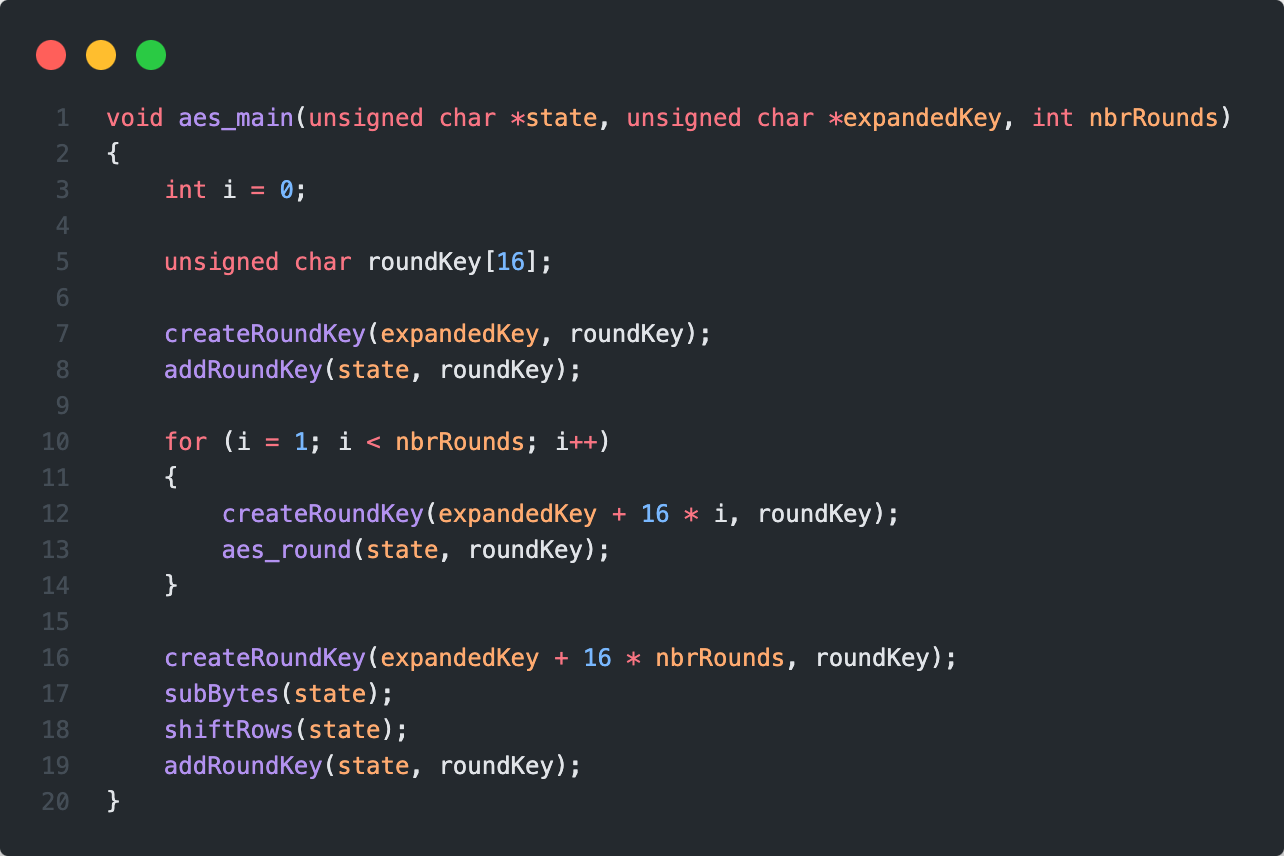
\includegraphics[width=0.8\textwidth]{cipher.png}
%     \caption{$\cipher$ C code}
% \end{figure}

% \begin{figure}[ht]
%     \centering
%     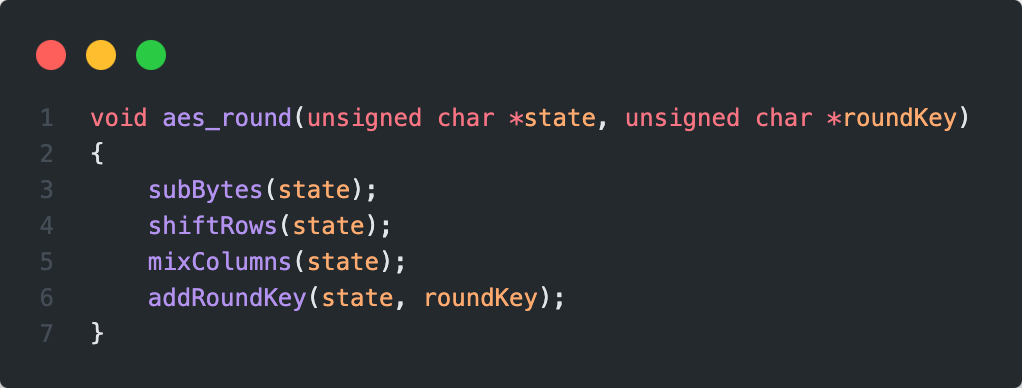
\includegraphics[width=0.8\textwidth]{round.png}
%     \caption{Round C code}
% \end{figure}

\cipher 의 입력 데이터, 라운드 수, 라운드 키 세 개이다. 데이터는 16 바이트 선형
배열로 표현되는 블록이며, 라운드 수는 해당 AES 인스턴스에 대한 라운드 수이다.
예를 들어, \aes{128}의 \cipher 함수는 다음과 같이 표현된다.
$$
    \cipher(\pt, 10, \KE(key)).
$$

\cipher 에서 라운드는 \sb, \sr, \mc, \ar \ 네 가지 바이트 단위 변환을 포함한다.
이 네 가지 변환 규격은 하위 절에서 설명한다.

첫 번째 단계(line 2)는 입력을 $\state$ 에 복사한다. 초기 라운드 키 추가(line 3)
후, $\state$는 $\nr$ 번의 라운드 함수 변환을 거친다(line 4 to 9). 마지막
라운드(line 10 to 12)는 \mc 변환이 생략된다는 점에서 이전 라운드들과 다릅니다.
최종 \state 는 출력으로 반환된다(line 13).


\subsubsection{AddRoundKey}


% \begin{figure}[ht]
%     \centering
%     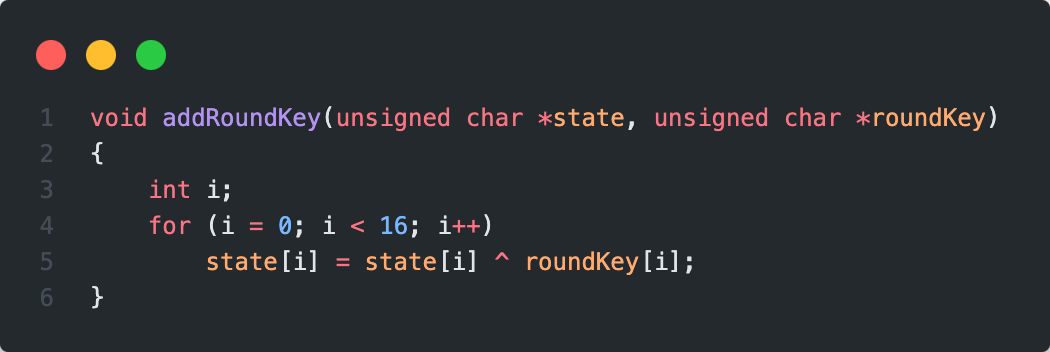
\includegraphics[width=0.8\textwidth]{addroundkey.png}
%     \caption{$\ar$ C code}
% \end{figure}

\ar 은 $\state$에 라운드 키를 적용하여 비트 단위 XOR 연산을 수행하는 변환이다. 
% 각 라운드 키는 키 스케줄로부터 4개의 워드로 구성되며, 이 워드들은 상태의 각 열과 결합된다.
과정은 다음과 같이 표현된다.
$$
    [s'_{0, c}, s'_{1, c}, s'_{2, c}, s'_{3, c}]
     = [s_{0, c}, s_{1, c}, s_{2, c}, s_{3, c}]
     \xor [w_{0, 4r + c}, w_{1, 4r + c} , w_{2, 4r + c}, w_{3, 4r + c}],
     \for 0 \le c < 4.
$$

\ar 는 \cipher 에서 총 $\nr + 1$번 호출된다. 첫번째 라운드 함수 적용 전에 한 번,
그리고 $\nr$ 번의 라운드에서 한 번씩 호출된다.


\subsubsection{SubBytes}


% \begin{figure}[ht]
%     \centering
%     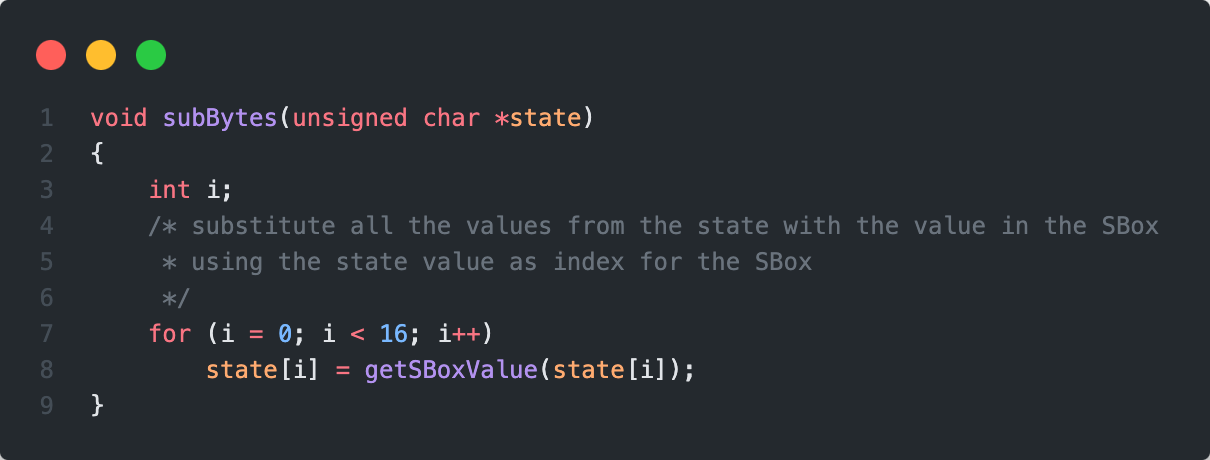
\includegraphics[width=0.8\textwidth]{subbytes.png}
%     \caption{$\sb$ C code}
% \end{figure}

% \begin{figure}[ht]
%     \centering
%     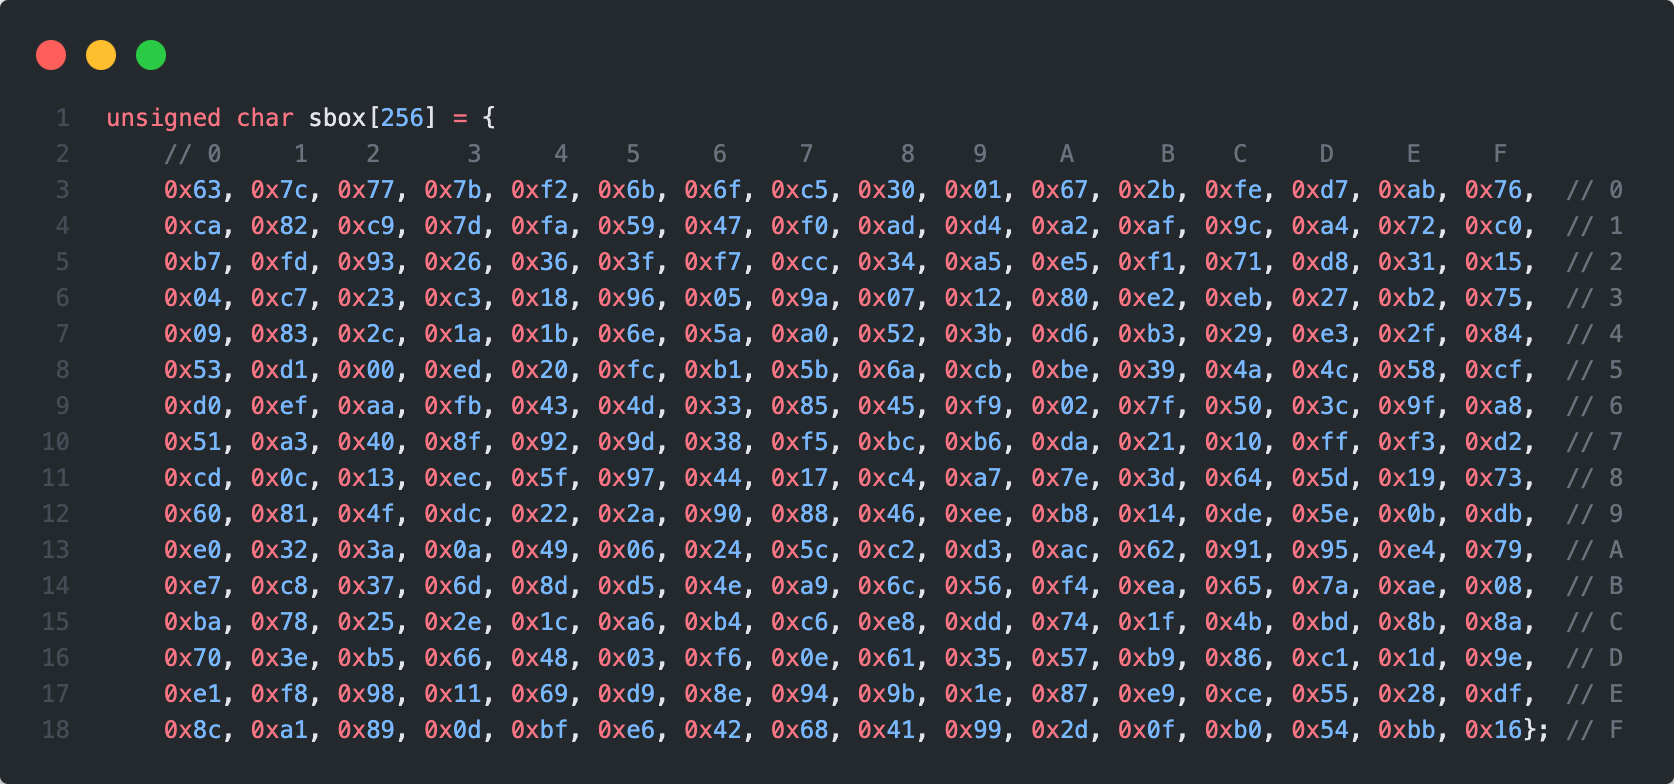
\includegraphics[width=0.8\textwidth]{sbox.png}
%     \caption{$\SBox$ C code}
% \end{figure}

\sb 는 $\state$에 대해 가역적이고 비선형적인 변환을 수행하는 함수로, 각 바이트에
대해 \SBox 라고 불리는 치환 테이블을 독립적으로 적용한다. 입력 바이트 $b$를 \SBox
에 입력한다고 하자. 출력 바이트 $b'$은 다음 두 가지 변환을 조합하여 구성된다.

\begin{itemize}
    \item 중간값 $\tilde{b}$을 다음과 같이 계산한다.
    % 여기서 b^{-1}은 ...에서 설명된 대로 b의 곱셈 역원이다.
    $$
    \tilde{b} = \begin{cases} 
            \hex{00}, & \IF b = \hex{00} \\ b^{-1}, & \IF b \neq \hex{00}. 
        \end{cases}
    $$
    \item $\tilde{b}$의 비트에 다음 아핀 변환을 적용해 $b'$의 비트를 생성한다.
    (이 때, $c$는 상수 바이트로, $c = \texttt{0b01100011}$이다.)
    $$
    b'_i = \tilde{b}_i 
        \xor \tilde{b}_{(i+4) \Mod 8} 
        \xor \tilde{b}_{(i+5) \Mod 8} 
        \xor \tilde{b}_{(i+6) \Mod 8} 
        \xor \tilde{b}_{(i+7) \Mod 8} \xor c_i.
    $$
    
\end{itemize}


\subsubsection{Shiftrows}


% \begin{figure}[ht]
%     \centering
%     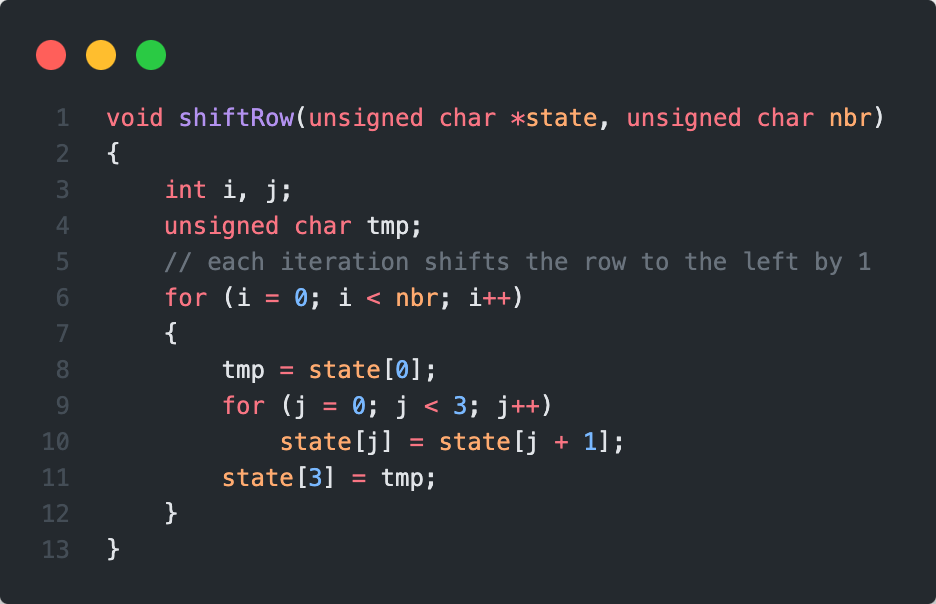
\includegraphics[width=0.8\textwidth]{shiftrow.png}
%     \caption{$\sr$ C code}
% \end{figure}

\sr 은 $\state$에서 마지막 세 개의 행에 속한 바이트들이 순환적으로 이동하는 변환이다.
각 행에서 바이트가 이동하는 횟수는 인덱스 $r$에 따라 달라지며, 다음과 같이 정의된다.
$$
    s'_{r,c} = s_{r, (c+r) \Tmod 4} \for 0 \leq r < 4 \Tand 0 \leq c < 4.
$$

이 변환은 각 바이트를 해당 행에서 $r$만큼 왼쪽으로 이동시키고, 왼쪽에서 밀려난
바이트를 행의 오른쪽 끝으로 순환 시키는 것이다. 단, 첫번째 행은 변환되지 않고
그대로 유지된다.


\subsubsection{Mixcolumns}


% \begin{figure}[ht]
%     \centering
%     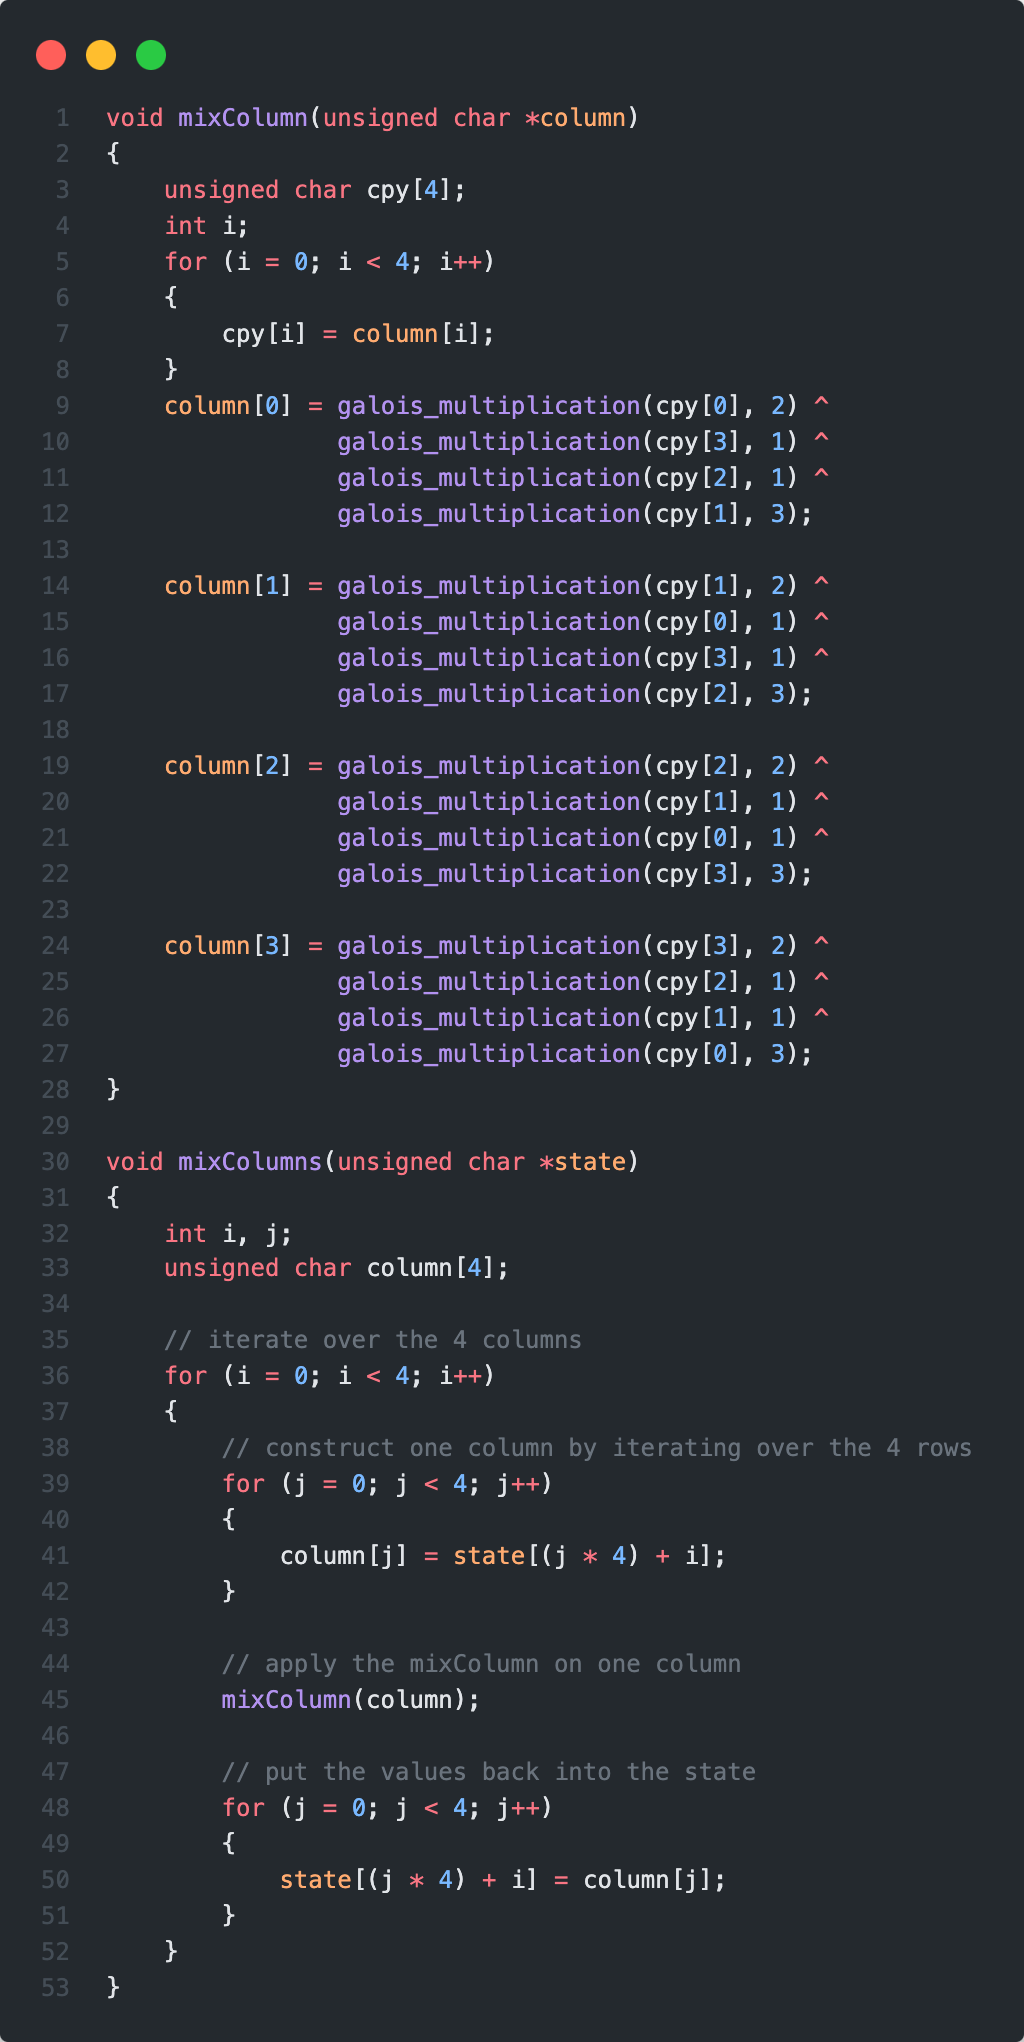
\includegraphics[width=0.55\textwidth]{mixcolumn.png}
%     \caption{$\mc$ C code}
% \end{figure}

\mc 는 $\state$의 각 열을 고정된 행렬과 곱하는 변환이다. 과정은 다음과 같다.
$$
    \begin{bmatrix}
        s'_{0,c} \\
        s'_{1,c} \\
        s'_{2,c} \\
        s'_{3,c}
    \end{bmatrix}
     = \begin{bmatrix}
        \hex{02} & \hex{03} & \hex{01} & \hex{01} \\
        \hex{01} & \hex{02} & \hex{03} & \hex{01} \\
        \hex{01} & \hex{01} & \hex{02} & \hex{03} \\
        \hex{03} & \hex{01} & \hex{01} & \hex{02}
    \end{bmatrix} 
    \begin{bmatrix}
        s_{0,c} \\
        s_{1,c} \\
        s_{2,c} \\
        s_{3,c}
    \end{bmatrix} \for 0 \le c < 4.
$$

% $$
%     \begin{bmatrix}
%         s'_{0,c} \\
%         s'_{1,c} \\
%         s'_{2,c} \\
%         s'_{3,c}
%     \end{bmatrix}
    
%     \begin{bmatrix}
%         02 & 03 & 01 & 01 \\
%         01 & 02 & 03 & 01 \\
%         01 & 01 & 02 & 03 \\
%         03 & 01 & 01 & 02
%     \end{bmatrix}

%     \begin{bmatrix}
%         s_{0,c} \\
%         s_{1,c} \\
%         s_{2,c} \\
%         s_{3,c}
%     \end{bmatrix}

%     \for 0 \leq c < 4.
% $$


\subsection{InvCipher} 

\begin{algorithm}
    \caption{\invcipher}
    \begin{algorithmic}[1]
    \Require $\In, \nr, \Rk$ \Comment{$\Rk = \KE(\key)$}
    \Ensure $\Out$ 
    \Procedure{InvCipher}{$\In, \nr, \Rk$}
    \State $\St \gets \In$
    \State $\St \gets \ar(\St, \Rk_{[4\nr: 4(\nr + 1)]})$
    \For{$i = 1$ to $\nr - 1$}
        \State $\St \gets \isr(\St)$
        \State $\St \gets \isb(\St)$
        \State $\St \gets \ar(\St, \Rk_{[4i: 4(i + 1)]})$
        \State $\St \gets \imc(\St)$
    \EndFor
    \State $\St \gets \isr(\St)$
    \State $\St \gets \isb(\St)$
    \State $\St \gets \ar(\St, \Rk_{[0:4]})$
    \State $\Out \gets \St$
    \State \Return $\Out$
    \EndProcedure
    \end{algorithmic}
\end{algorithm}

\invcipher 는 \cipher 의 변환들이 역순으로 실행된다. $\state$의 역변환은 \ar,
\isb, \isr, \imc 으로 구성되며, \ar 을 제외한 각 변환은 하위 절에서 설명한다.


\subsubsection{InvSubBytes}


$\isb$는 $\sb$의 역연산이다. $\state$의 각 바이트에 $\sb$의 역함수인 $\iSBox$가
적용된다. 즉, $\iSBox$는 $\SBox$의 입력과 출력의 역할이 바뀌어 생성된다.


\subsubsection{InvShiftRows}


\isr 는 $\sr$의 역연산이다. $\state$의 마지막 세 개의 행에 있는 바이트들은 다음과 같이 순환 이동한다.
$$
    s'_{r, c} = s_{r, (c - r) \Tmod 4} \for 0 \le r < 4 \Tand 0 \le c < 4.
$$

이 변환은 각 바이트를 해당 행에서 $r$ 칸 씩 오른쪽으로 이동시키고, 오른쪽 끝에서
밀려난 $r$ 개의 바이트를 왼쪽 끝으로 순환 이동시킨다. 이 때, 첫 행은 변경되지
않는다.


\subsubsection{InvMixColumns}


\imc 는 \mc 의 역연산이다. \imc 는 $\state$ 에 고정된 행렬을 곱한다. 과정은 다음과 같다.
$$
    \begin{bmatrix}
        s'_{0,c} \\
        s'_{1,c} \\
        s'_{2,c} \\
        s'_{3,c}
    \end{bmatrix}
     = \begin{bmatrix}
        \hex{0e} & \hex{0b} & \hex{0d} & \hex{09} \\
        \hex{09} & \hex{0e} & \hex{0b} & \hex{0d} \\
        \hex{0d} & \hex{09} & \hex{0e} & \hex{0b} \\
        \hex{0b} & \hex{0d} & \hex{09} & \hex{0e}
    \end{bmatrix} 
    \begin{bmatrix}
        s_{0,c} \\
        s_{1,c} \\
        s_{2,c} \\
        s_{3,c}
    \end{bmatrix} \for 0 \le c < 4.
$$


\subsection{KeyExpansion}


\KE 은 키를 적용하여 $4 (\nr + 1)$개의 워드를 생성하는 함수이다.
따라서, \cipher 및 \invcipher 에서 \ar 를 $\nr + 1$ 번 적용하기 위해 4개의 워드
씩 생성된다. 이 함수의 출력은 $w_{[0:4(\nr + 1)]}$로 표시되는 선형 배열들의 워드들로 구성된다.

\KE 은 $1 \le j \le 10$ 범위에서 $\rc[j]$로 표시되는 10개의 고정된 워드를
호출한다. 이 10개의 워드를 라운드 상수라고 한다. $\rc[j]$ 값은 아래 표와 같다.
\begin{figure}[ht]
    \center
    \begin{tabular}{cccc}
        \hline
        \hline
        \rc[1]: & [\hex{01}, \hex{00}, \hex{00}, \hex{00}] & \rc[6]: & [\hex{20}, \hex{00}, \hex{00}, \hex{00}] \\
        \rc[2]: & [\hex{02}, \hex{00}, \hex{00}, \hex{00}] & \rc[7]: & [\hex{40}, \hex{00}, \hex{00}, \hex{00}] \\
        \rc[3]: & [\hex{04}, \hex{00}, \hex{00}, \hex{00}] & \rc[8]: & [\hex{80}, \hex{00}, \hex{00}, \hex{00}] \\
        \rc[4]: & [\hex{08}, \hex{00}, \hex{00}, \hex{00}] & \rc[9]: & [\hex{1b}, \hex{00}, \hex{00}, \hex{00}] \\
        \rc[5]: & [\hex{10}, \hex{00}, \hex{00}, \hex{00}] & \rc[10]: & [\hex{36}, \hex{00}, \hex{00}, \hex{00}] \\
        \hline
        \hline
    \end{tabular}
\end{figure}

$\aes{128}$은 10개의 라운드 키를 생성할 때 마다 고유한 라운드 상수가 호출되고,
\aes{192} 와 \aes{256}은 각 처음 8개와 7개의 라운드 상수를 호출한다.

\rc[j]의 최상위 바이트 값은 다항식 형태로 $x^{j-1}$이다. $j > 0$인 경우, 이러한
바이트 값은 $x^{j-1}$로 표현된 바이트에 $\XT$ 연산을 반복적으로 생성할 수 있다.

\KE 에서는 다음 두 가지 변환을 사용한다.
\begin{itemize}
    \item $\SW$: 4 바이트 입력 워드를 $[a_0, a_1, a_2, a_3]$라고 할 때, 다음과 같다.
    $$
        \SW([a_0, a_1, a_2, a_3]) = [\SBox(a_0), \SBox(a_1), \SBox(a_2), \SBox(a_3)].
    $$
    \item $\RW$: 위와 같은 입력 워드에 대해, 다음과 같다.
    $$
        \RW([a_0, a_1, a_2, a_3]) = [a_1, a_2, a_3, a_0].
    $$
\end{itemize}

\begin{algorithm}
    \caption{\KE}
    \begin{algorithmic}[1]
    \Require 키 $K$
    \Ensure 라운드 키 $\Rk$ 
    \Procedure{KeyExpansion}{$K$}
        \For{$i = 0$ to $\nk - 1$}
            \State $\Rk_i \gets K_i$
        \EndFor
        \For{$i = \nk$ to $4\nr + 3$}
            \State $t \gets \Rk_{i-1}$
            \If{$i \Tmod \nk = 0$}
                \State $t \gets \SW(\RW(t)) \xor \rc[i/\nk]$
            \ElsIf{$\nk > 6 \Tand i \Tmod \nk = 4$} \Comment{\aes{256}에서만 동작}
                \State $t \gets \SW(t)$
            \EndIf
            \State $\Rk_i \gets \Rk_{i - \nk} \xor t$
        \EndFor
        \State \Return $\Rk$
    \EndProcedure
    \end{algorithmic}
\end{algorithm}

키 확장 알고리즘은 위와 같다. 확장된 키의 첫 $\nk$ 워드는 키 $\key$이다. 이후 각
워드 $w[i]$는 이전 워드 $w[i-1]$ 및 $\nk$ 앞 워드 $w[i - \nk]$를 사용하여
재귀적으로 생성한다. 이를 수식으로 나타내면 다음과 같다.
\begin{itemize}
    \item 만약 $i$가 $\nk$의 배수면, $w[i]$를 다음과 같이 계산한다.
    $$
        w[i] = w[i - \nk] \xor \SW(\RW(w[i-1])) \xor \rc[i/\nk].
    $$
    \item 아니라면, 다음과 같이 계산한다. 
    $$
        w[i] = w[i - \nk] \xor w[i - 1].
    $$
    단, \aes{256}에서, $i + 4$가 8의 배수일 때는 다음과 같이 계산한다.
    $$
        w[i] = w[i - \nk] \xor \SW(w[i-1]).
    $$
\end{itemize}

\end{document}
